\section{Methods}
\subsection{Datasets, selection units and signal processing}
GRABMyo v1.1.0 contains \GRABMyoParticipants\ able-bodied participants recorded over \GRABMyoSessions\ days with an EMGUSB2+ amplifier at 2048 Hz \citep{pradhan2022multiday,jiang2024grabmyo}. Source-reported demographics were \GRABMyoMale\ male and \GRABMyoFemale\ female, age \GRABMyoAgeMean\ $\pm$ \GRABMyoAgeSD\ years. The forearm montage has sixteen monopolar sites in two rings (figure~\ref{fig:montage}); each site supplies one channel, so electrode and channel selection coincide here. Counts refer only to these signal recording sites; reference and ground requirements are not evaluated. The primary task uses sixteen active gestures, excluding rest. All \GRABMyoFilesVerified\ distributed files matched published checksums, and \GRABMyoRecords\ records were processed. Source demographics and the official gesture dictionary are provided with the reproducibility package.

Signals were filtered at 20--450 Hz using a Butterworth band-pass with SciPy order argument 4 (eight poles per pass), applied forward and backward for zero phase, followed by a forward--backward 50 Hz notch ($Q=30$). They were then divided into 250 ms windows with 50\% overlap within trial boundaries. The non-causal filter limits the analysis to offline use. Each channel supplied mean absolute value, RMS, variance, waveform length, zero crossings, slope sign changes, integrated EMG, Willison amplitude, mean frequency and median frequency. The active-task cache contains \GRABMyoActiveWindows\ windows with 160 features each.

Count-feature thresholds followed a common rule: 1.15 times the median absolute signal first difference, rounded to one significant figure. Historically, the monopolar threshold ($10^{-2}$ mV) was derived from 54 unfiltered records from six participants before LOSO. It was not estimated separately within each outer fold. Subsequent exclusion checks reproduced the identical rounded threshold in all \LOOMonoFolds\ folds. Thus the stored features are invariant to this particular exclusion, but the original development sequence should not be described as fully isolated. Fold-specific feature means and standard deviations, classifier fitting and attribution ranking exclude the outer test participant.

NinaPro DB5 was analyzed separately: \DBFiveSubjects\ participants, two Myo armbands, sixteen channels sampled at 200 Hz and exercise 1's twelve finger movements \citep{pizzolato2017comparison}. Refined labels determine movement segments. Filtering was effectively \RevDBFiveBandLow--\RevDBFiveBandHigh\ Hz without a notch; the requested \RevDBFiveBandRequestedHigh\ Hz upper limit was clipped by the shared implementation to $0.45f_s-1$ Hz. Complete raw reconstruction of all saved DB5 feature rows verified this implemented cutoff; the earlier 95 Hz description was a reporting error. The 250 ms windows contain 50 samples. The threshold is seven quantization steps in the stored integer representation; every participant-exclusion check reproduced it. Source-reported DB5 demographics were \DBFiveMale\ male and \DBFiveFemale\ female, age \DBFiveAgeMean\ $\pm$ \DBFiveAgeSD\ years. Sex is reported as recorded in the source datasets; no sex-specific effect is estimated. No anatomical correspondence between DB5 and GRABMyo channel numbers is assumed.

\paragraph{Ethics} This is a secondary analysis of publicly distributed, de-identified recordings, with no new recruitment or recording. Original study approvals and consent are described in the dataset publications. [AUTHOR INPUT REQUIRED: institutional determination or exemption for this secondary analysis remains unresolved.]

\subsection{Outer evaluation and classifier budgets}
Each outer LOSO fold reserves all observations of one participant $p$. For cross-fitted attribution, an inner five-fold GroupKFold partitions only the other participants (figure~\ref{fig:workflow}). Inner feature standardization uses inner-training observations only; final reduced models use the corresponding outer-training statistics. No outer test observations enter fitting or rankings.

The primary reduction curve uses XGBoost with 300 boosting rounds, maximum depth 6, learning rate 0.1, row and column subsampling 0.8, histogram tree construction and fixed seed 20260728. Its multiclass soft-probability objective produces probabilities whose argmax gives the predicted class. For the primary curve, final models across all counts and fixed penalty rankings within an outer fold use the same stratified sample of 200,000 outer-training windows. Models are retrained from scratch on the selected features. Selected features retain their original column order.

Training budgets differ across historical tracks: the full-array XGBoost classifier context uses all training windows, the primary curve uses 200,000, and the random-selection comparison uses 50 boosting rounds and 150,000. The full-array SVM uses 40,000 windows; random forest uses 200,000. These are budget-limited comparators, not proven lower bounds or matched classifier-capacity experiments. Budgets were calibrated using two outer-fold outcomes. The internally dated analysis plan followed an earlier pilot; no independent registration or Git commit authenticating its date is available. These development exposures qualify claims of wholly prospective evaluation.

\begin{figure}[htbp]\centering
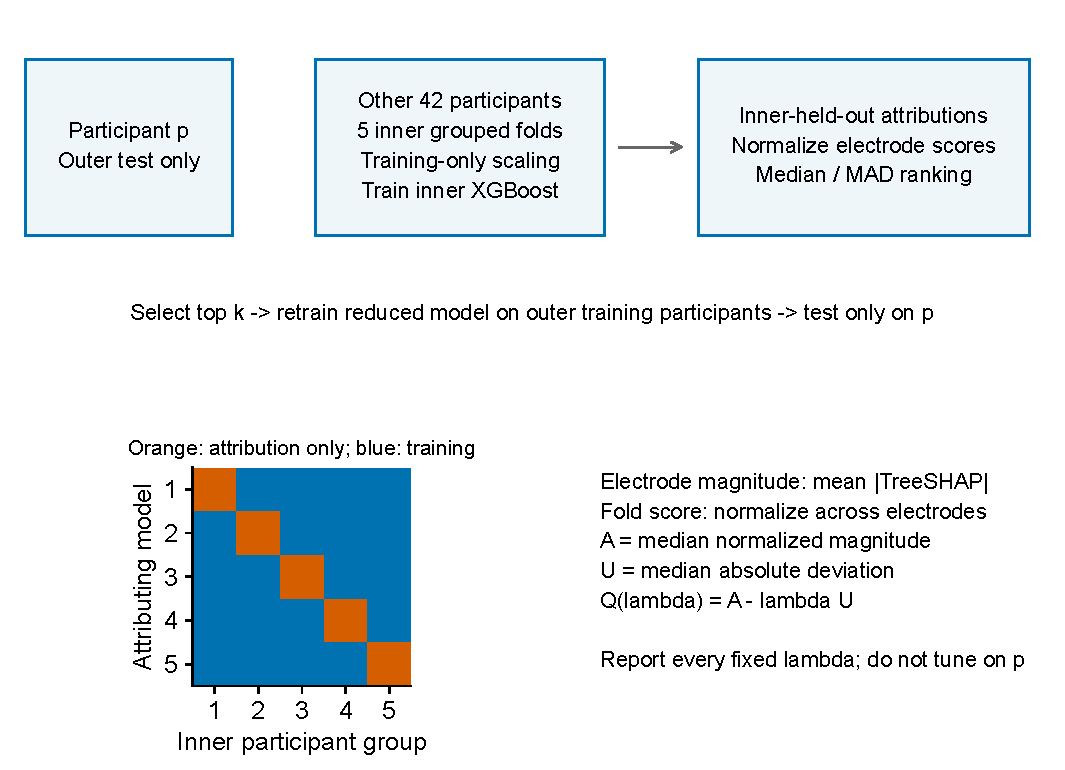
\includegraphics[width=\textwidth]{../figures/vector/fig2_crossfit.pdf}
\caption{Participant access in the nested procedure. Each inner attributing model excludes the participants on whom its attributions are evaluated. The outer participant is reserved until final reduced-model testing. This diagram describes fold-specific scaling, fitting and ranking; historical threshold pooling and budget calibration are separate development exposures documented in the text.}
\label{fig:workflow}\end{figure}

\subsection{Cross-fitted attribution and its participant-level extension}
Inner XGBoost models use at most 200,000 training windows sampled uniformly without replacement after participant splitting. Their standardization statistics use the full inner-training pool, not the capped model-fit sample. Exact tree-path-dependent TreeSHAP contributions are computed on raw class margins for at most 20,000 inner-held-out windows. For window $i$ and electrode $c$, absolute contributions are averaged across classes $g$ and its ten features $f$:
\begin{equation}\Phi_{i,c}=\frac{1}{GF}\sum_{g=1}^G\sum_{f=1}^F|\phi_{i,g,c,f}|.\end{equation}
The mean over inner-held-out windows is normalized across electrodes to give the inner-fold score $I_{j,c}$. The central magnitude and unscaled median absolute deviation are
\begin{equation}A_c=\operatorname{median}_j I_{j,c},\quad U_c=\operatorname{median}_j|I_{j,c}-A_c|,\quad Q_c(\lambda)=A_c-\lambda U_c.\end{equation}
All fixed penalties $\lambda\in\{0,0.25,0.5,1\}$ are reported, with lower electrode index breaking ties. No penalty is chosen using outer scores. The unpenalized ranking is called cross-fitted SHAP; the positive penalties assess stability regularization.

Pooling people within five inner folds can suppress person-level heterogeneity. A post-hoc extension therefore computes the median and MAD over normalized individual attribution vectors of all 42 outer-training participants. These vectors share five fitted inner models; their dispersion is descriptive heterogeneity, not a standard error. All penalties and counts are evaluated under the unchanged primary protocol. Exact matching participant/subset fits may be reused with source-row provenance; new subsets require new fits. A historical source-hash mismatch is preserved in the audit, and current reporting uses an isolated refit with current input fingerprints. After observing the penalty results, a descriptive audit compared selected physical site sets and Jaccard similarity at every fixed penalty and count. It added no model fits or inferential tests and did not choose a penalty.

\subsection{Primary endpoint and participant-level inference}
Macro-F1 is the unweighted mean of the gesture F1 scores for each held-out participant. For count $k$, the paired change is $\Delta_{p,k}=\mathrm{F1}_{p,k}-\mathrm{F1}_{p,16}$. The predefined primary engineering tolerance is $\delta=0.02$ on the 0--1 scale. The historical decision rule requires the lower 95\% percentile-bootstrap bound on the participant mean change to exceed $-\delta$; $k^*$ is the smallest qualifying count below sixteen. Sensitivity margins are 0.01 and 0.03. This criterion concerns mean recognition performance, has no established clinical interpretation and does not imply equivalence or individual preservation.

The participant is the statistical unit: 43 for GRABMyo, ten for DB5 and 21 or 22 test participants for split-layout checks. Bootstrap intervals use 10,000 resamples of paired participant scores with seed 20260728. They are conditional on the observed fitted LOSO models. Overlapping training cohorts and the lack of refitting within every bootstrap mean these intervals do not capture all new-cohort training uncertainty \citep{bengio2004variance}.

The original Holm procedure used the fraction of unshifted bootstrap mean differences at or below $-\delta$, with a Monte Carlo floor. This is a percentile-tail quantity rather than a bootstrap distribution generated under the null. We preserve it and additionally report an exploratory, null-centred studentized bootstrap \citep{davison1997bootstrap}. For $d_p=\Delta_{p,k}$, residuals $d_p-\bar d$ are resampled, their studentized means are compared with $(\bar d+\delta)/(s_d/\sqrt n)$, and the upper-tail probability uses a plus-one correction. Holm adjustment covers the fifteen reduced-count tests at one-sided $\alpha=0.025$, separately for each condition, margin and penalty. No seed or margin is chosen from results.

Paired secondary contrasts use Wilcoxon signed-rank tests and participant mean-change percentile intervals. These address different estimands: signed ranks are not a test of the mean. Holm families are stated explicitly; a non-significant contrast is not evidence of equivalence. The detailed historical secondary families were specified after their underlying results became available and are labeled secondary rather than prospectively confirmatory.

\subsection{Selection comparators and attribution diagnostics}
Historical lighter-model comparisons use random subsets, cross-fitted SHAP, stability-regularized SHAP ($\lambda=0.5$), feature-wise permutation, mutual information and geometric farthest-point selection. Random selection uses 100 subsets per participant at counts 4, 6 and 8, and 500 at count 12. Eight attribution-versus-mean-random contrasts receive Holm correction. Historical permutation uses one model fitted on 20,000 windows and three feature-wise permutations on 8,000 non-overlapping windows from the same outer-training participant pool. Its 40,000-window ranking pool was standardized before the window split; this was not participant-disjoint inner validation. The outer test participant remained excluded. SHAP instead uses the participant-disjoint cross-fitting above. Thus shared final evaluation does not equalize their selection resources or validation designs.

New exploratory geometry12 testing uses the primary 300-round, 200,000-window protocol, the same outer training sample and full16 reference. Geometric selection uses the fixed two-ring topology, nominal 24 cm circumference and 2 cm separation, starts at F1 and successively maximizes distance from selected sites; ties favor the lower index. It is not tuned to participant outcomes. After the geometry12 results were known, an exploratory amendment extended this fixed ordering to every count under the unchanged primary protocol. The count-12 and full-array metrics were reused from the exact matched predictions, and remaining subsets were fitted separately.

A separate exploratory resource-matched comparison shares five inner models between SHAP and grouped-electrode permutation, with up to 200,000 uniformly sampled training and 2,000 validation windows per fold. Equal validation quotas represent every inner-held-out participant. All ten features of one electrode are permuted jointly within each participant, three repeats, scoring the equally weighted mean participant Macro-F1 loss. Signed losses are retained, normalized by their summed absolute magnitude, and aggregated by the median across inner folds. SHAP uses the identical observations and normalizes absolute contribution magnitudes. Final models at counts 6 and 12 use the primary protocol; two contrasts receive Holm correction. Measured training and selection times are reported separately. CPU RF fits overlapped with early folds of this experiment, so these are observed workstation timings rather than an isolated runtime benchmark. Because permutation grouping, participant-disjoint validation, scaler isolation and resources all differ from the historical method, this experiment does not isolate a budget effect.

Deletion with retraining uses the unpenalized primary ordering and compares removal of high-ranked, random and low-ranked electrodes using the lighter model. Its fifteen contrasts form one Holm family. This diagnostic tests predictive ranking relevance; it cannot identify causal muscles or validate an online controller.

\subsection{Participant and gesture degradation}
Primary full16, SHAP12 and geometry12 models were rerun to retain predictions indexed to the same canonical outer-test rows. Full16 and SHAP12 scores must reproduce the original curve within $10^{-6}$. Participant losses, quantiles, worst loss and the number exceeding the primary margin are descriptive. Gesture-specific F1 differences are paired over all participants, with Holm correction across sixteen gestures. Confusion changes average row-normalized confusion matrices within participants so people, rather than windows, receive equal weight. Gesture names follow the explicit numeric ordering in MotionSequence.txt.

\subsection{Sensitivity, transfer and fixed-layout scope}
Rest-inclusive recognition and 150/500 ms windows use raw-signal re-extraction and complete count curves with the primary 250 ms ranking held fixed. The 150 ms window is 307 samples with stride 153; 250/500 ms use 512/1024 samples and half-window strides. The same 200,000-window count does not equate recording duration across windows. A random-forest sensitivity uses the pre-existing 200-tree, minimum-leaf-size-2 configuration at counts 12 and 16, the unchanged XGBoost ranking and the same training sample. It tests those counts only and cannot establish a random-forest minimum count.

DB5 applies the procedure separately with its own sixteen-channel reference. Derived bipolar signals $B_j=F_j-F_{j+8}$ use eight aligned pairs, re-extracted features and the eight-pair reference; they are not physical bipolar-sensor measurements. Full-array cross-session analyses compare training on session 1 with testing on sessions 1--3, and training on sessions 1--2 with testing on session 3. They do not test a reduced layout under displacement, and the latter comparison confounds data quantity with session diversity.

Fixed-layout checks use odd-ID development/even-ID testing and the reverse, each deriving a layout using development participants only and the original five-fold median/MAD aggregation rule. Their inner and final models use all development windows with training-only standardization and the same 300-round classifier, rather than the primary curve's 200,000-window cap. The historical pooled feature thresholds also apply to these checks. The count of twelve had already been selected using the full cohort, so neither direction independently validates count selection. The layouts differ and must be reported separately. To quantify Monte Carlo decision sensitivity near the boundary, a post-hoc diagnostic repeated the original percentile bootstrap with 200 seeds drawn once from a generator initialized at 20260728, using 10,000 resamples for each seed. Every seed outcome is retained; the diagnostic never replaces the original seed or decision. No fresh, independently collected cohort with this montage was available. Feature redundancy and ranking-agreement diagnostics are documented in the Supplementary and machine-readable outputs; high outer-fold agreement is qualified by extensive training-set overlap.
